\chapter{Conclusion and Outlook}
\label{chap:conclusion-outlook}

Through a successive isolation of errors from the turbulence model (ref. Section~\ref{sec:comparative:zpg:wall-resolved-baselines}), the underlying wall-function closure theory (ref. Section~\ref{sec:comparative:zpg:cross-comparison}) and the spatial discretization (ref. Section~\ref{subsec:comparative:zpg:yplus-sensitivity}), novel findings and strong assessments to the accuracy of the aerothermal prediction of RANS with and without wall-functions was formed.
\par\medskip

Figure~\ref{fig:conclusion:overview-of-isolation-of-errors} shows the isolation of errors, from conventional coarse wall function mesh (top), to novel boundary layer informed mesh (middle) to additional posterior fitting of the closure (bottom), which then all in all results in the wall function CFD to be within the wall resolved result to within +-2\% - i.e. all the errors have been fully isolated and investigated (within error cancellation still being a thing also). 
\begin{figure}[H]
    \centering
    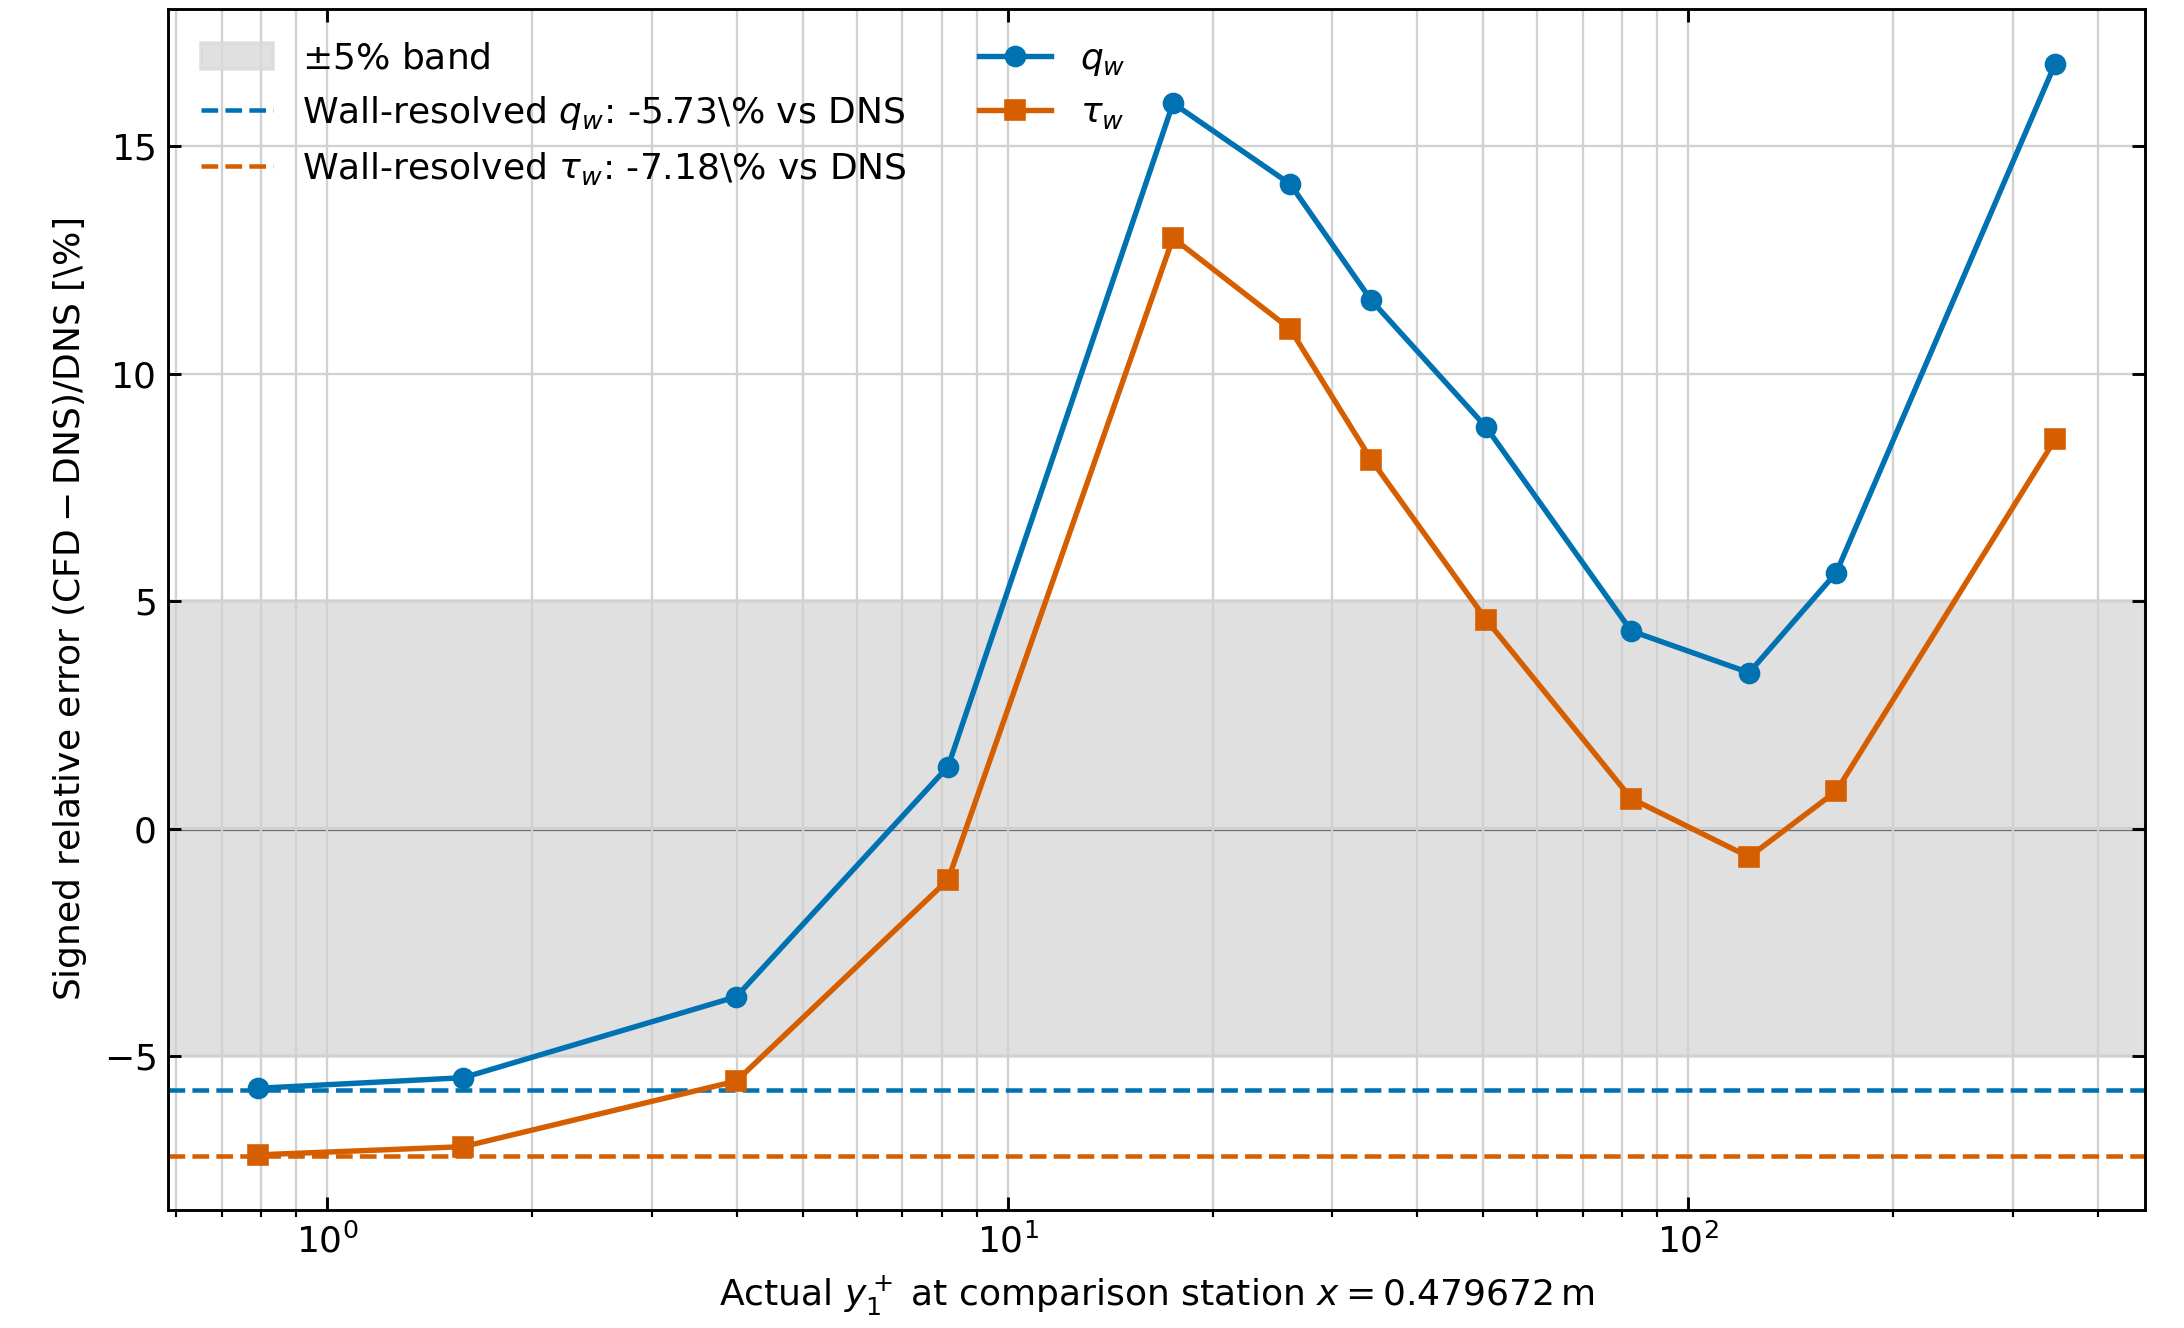
\includegraphics[width=\linewidth,height=.43\textheight,keepaspectratio]{07_Error_Isolation_Results/Figures/WallFunctions/04_ConvMesh_Li_LowHM3.png}
    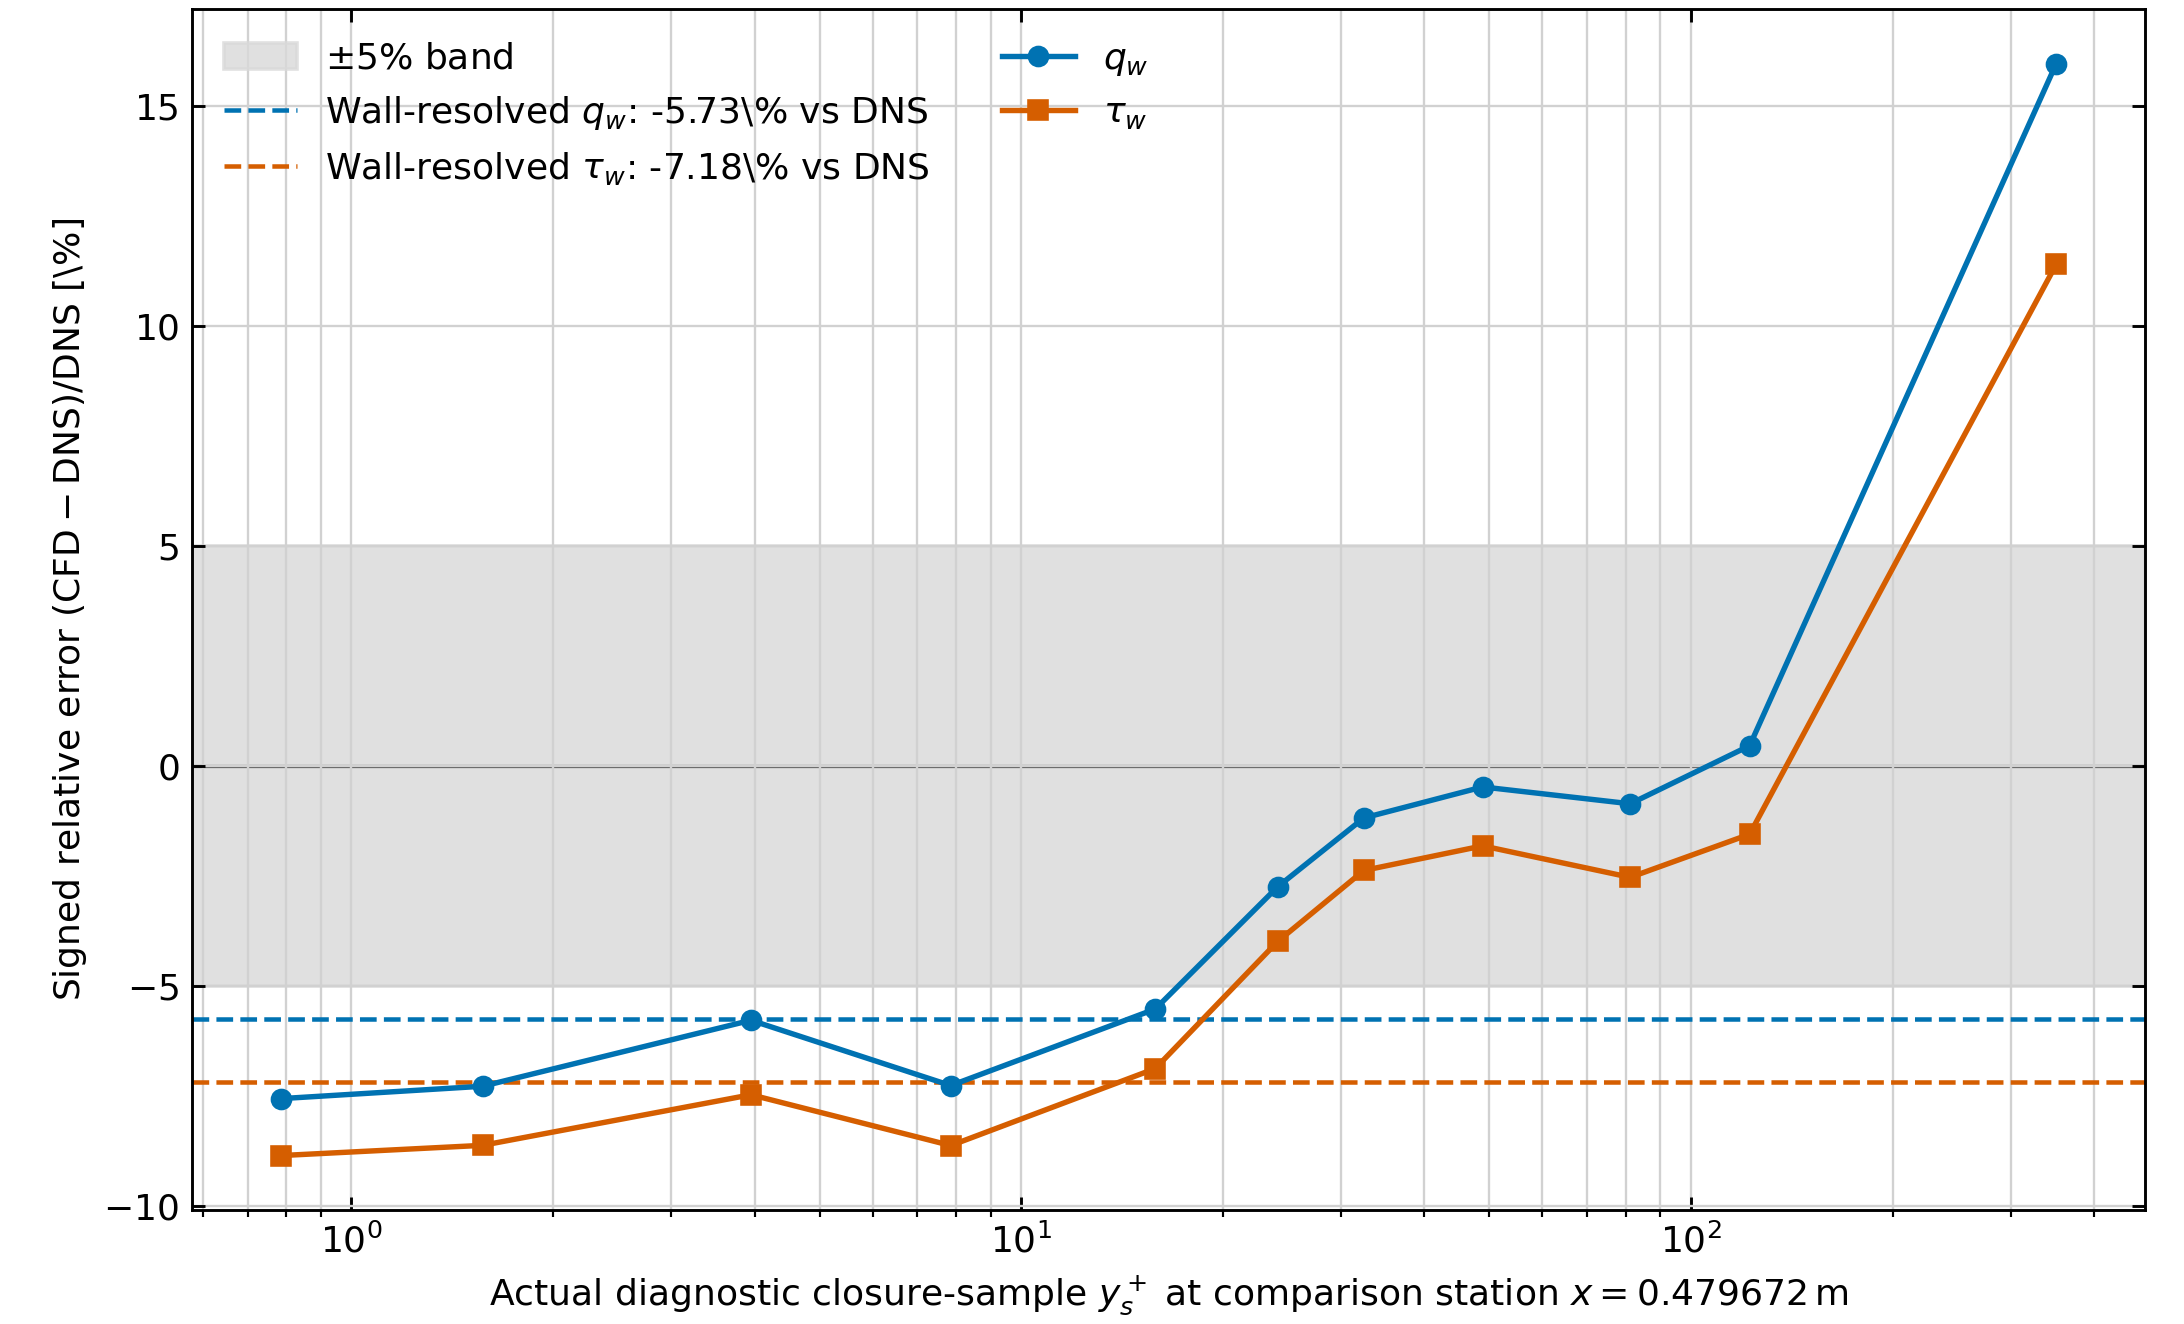
\includegraphics[width=\linewidth,height=.43\textheight,keepaspectratio]{07_Error_Isolation_Results/Figures/WallFunctions/04_3pctMesh_Li_LowHM3.png}
    \caption[Error-isolation sequence for LowH\_M3 with Li wall functions and SA.]{Error-isolation sequence for LowH\_M3 with Li wall functions and SA: conventional meshes (top), boundary layer-informed meshes (bottom), and fitted closures on informed meshes (continued). Signed wall heat-flux and shear-stress errors are relative to DNS; dashed lines show the wall-resolved SA baseline and shading marks the $\pm5\%$ DNS band. The abscissa is the first-cell location $y_1^+$ on conventional meshes and the sampling location $y_s^+$ on informed meshes.}
    \label{fig:conclusion:overview-of-isolation-of-errors}
\end{figure}
\begin{figure}[H]
    \ContinuedFloat
    \centering
    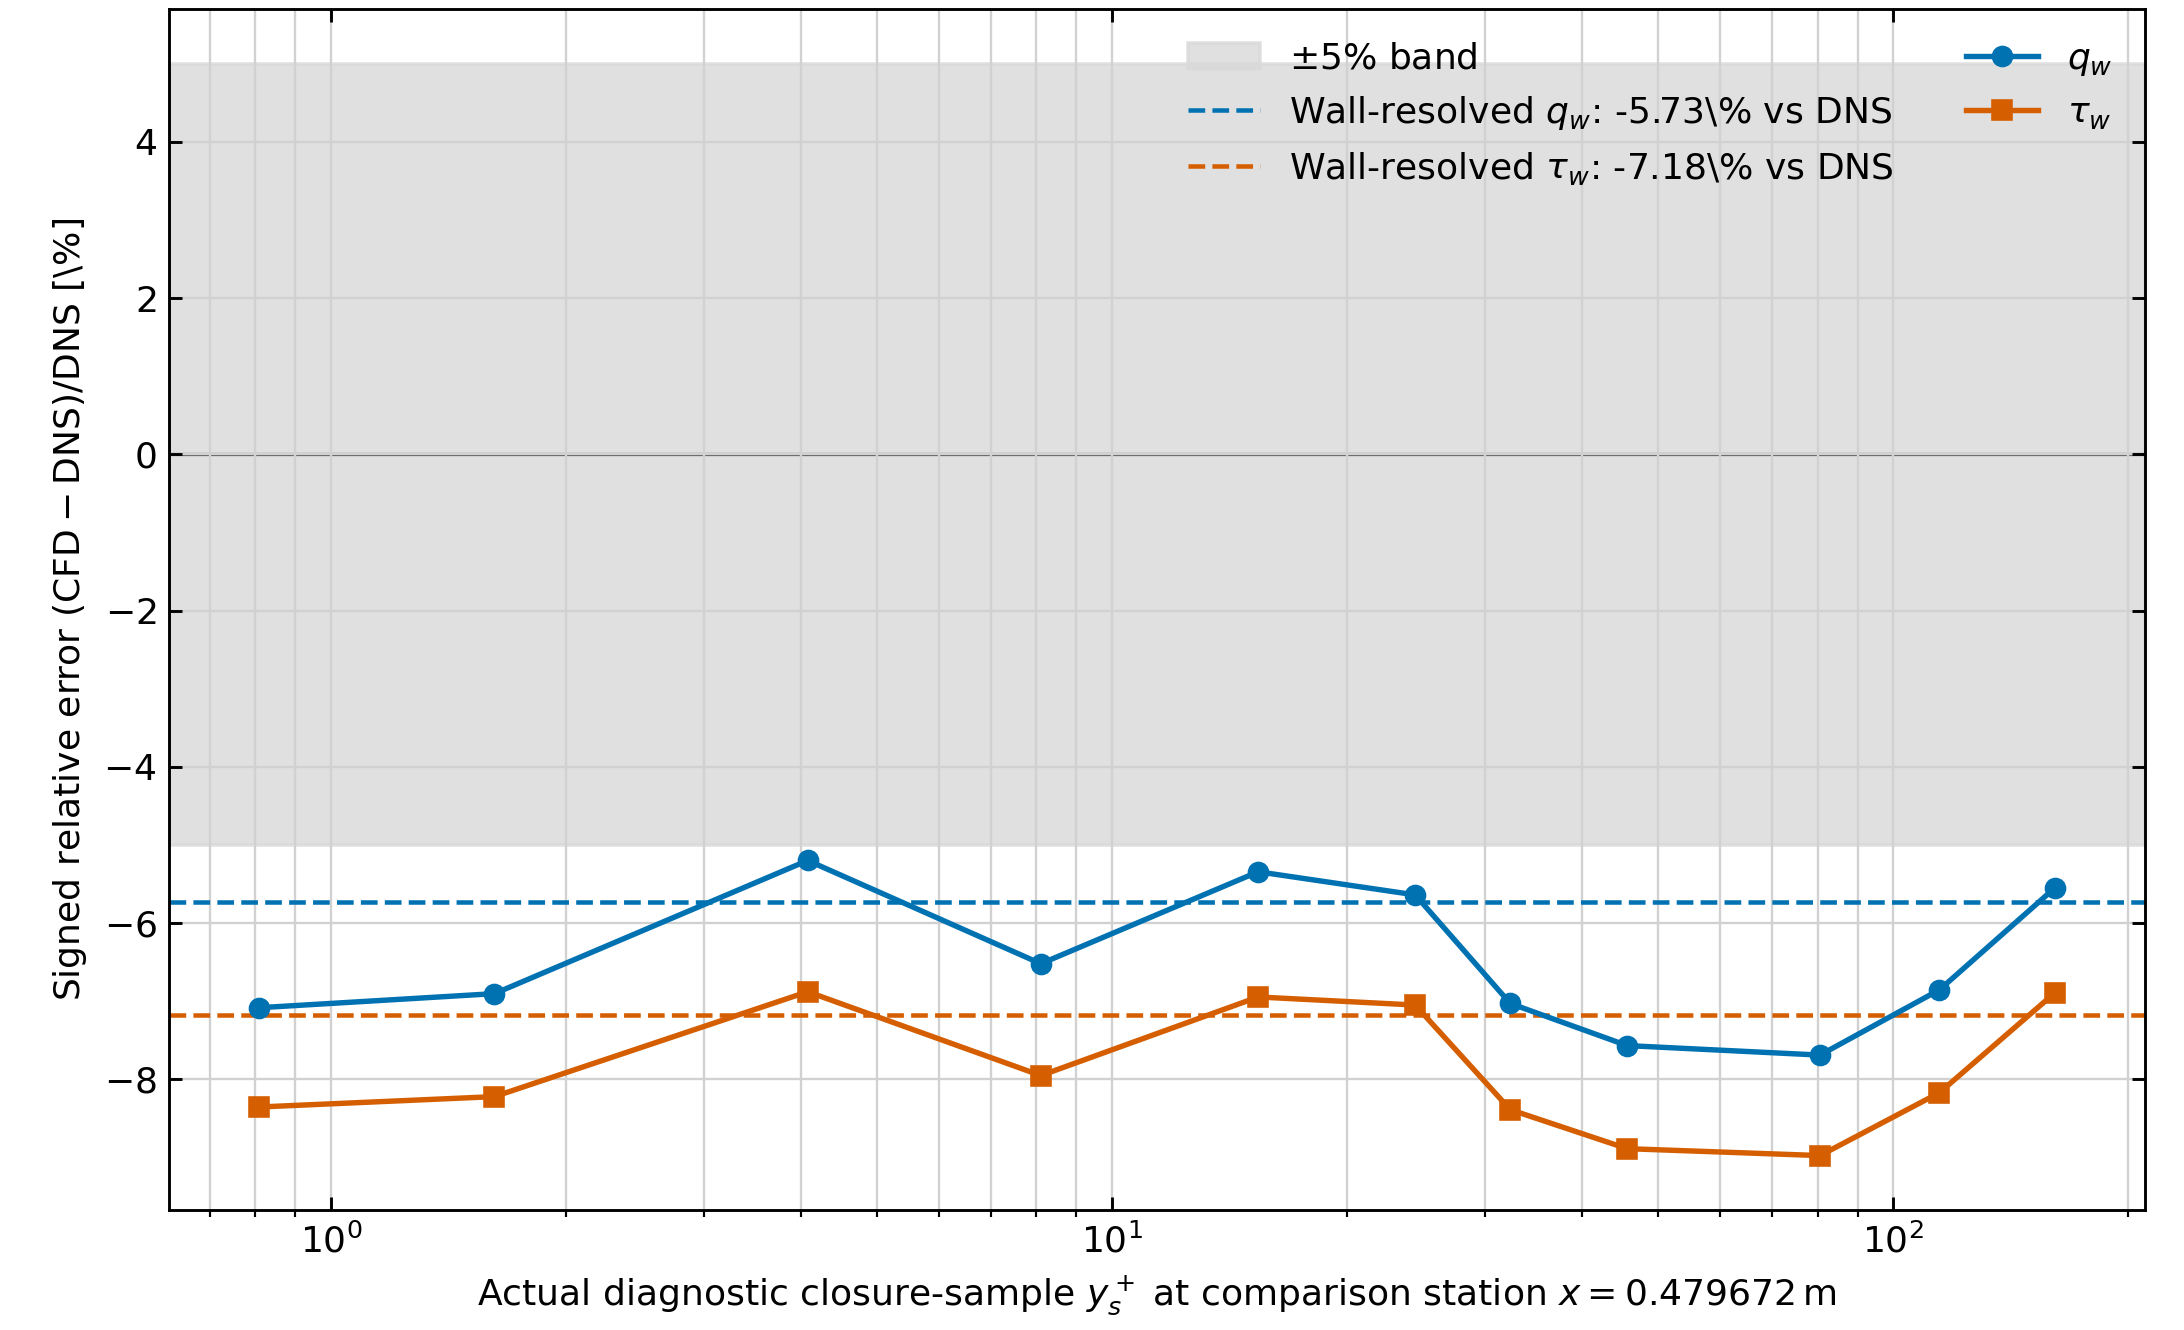
\includegraphics[width=\linewidth,height=.43\textheight,keepaspectratio]{07_Error_Isolation_Results/Figures/WallFunctions/04_3pctMesh_fitted_Li_LowHM3.png}
    \caption[]{(continued) Closures fitted to the wall-resolved SA reference recover its wall heat-flux and shear stress to within approximately $\pm2\%$ on the informed meshes. The baseline discrepancy from DNS remains.}
\end{figure}


\section{Summary}

The main contribution of this work is a novel boundary layer-informed mesh criterion, which is necessary for wall-function simulations of hypersonic cold-wall flat plates. It relates cell spacing to the local profiles, controlling internal-face gradient and transport-coefficient interpolation errors (Sections~\ref{subsec:comparative:zpg:mesh-criterion} and~\ref{subsec:comparative:zpg:informed-mesh}). This criterion also provides the basis for a proposed a-priori mesh-design approach, conditional on estimates of wall loads and wall/edge states (Section~\ref{subsec:comparative:zpg:apriori-mesh}).
\par\medskip

A-priori assessment, independently of coupled CFD, of the Li and Griffin wall-function closures was performed. Across the investigated adiabatic and cold-wall flat plates, relative shear-stress and heat-flux errors are of order \(\pm 10\%\) over the assessed inner-layer sampling range, with some larger deviations in some cases (Section~\ref{subsec:erriso:apriori-results}). This demonstrates promising closure accuracy, although reliance on reconstructed boundary layer-edge quantities introduces an additional sensitivity in CFD (Section~\ref{subsec:wall-functions:griffin:edge-detection}).
\par\medskip

The wall-resolved assessment of the Spalart--Allmaras and \(k\)--\(\omega\) SST turbulence models across twelve zero-pressure-gradient flat-plate cases reinforces existing evidence of their limitations in hypersonic cold-wall flows. Wall heat-flux and shear-stress predictions show substantial, case-dependent discrepancies from DNS, reaching approximately \(\pm 20\%\) (Section~\ref{subsec:comparative:zpg:wr-wall-fluxes}).
\par\medskip

Consistent with previous RANS assessments, both turbulence models were also found to struggle to reproduce the thermal profiles of hypersonic cold-wall boundary layers (Section~\ref{subsec:comparative:zpg:wr-profiles}). These profile discrepancies affect the wall functions that sample the RANS field (Section~\ref{subsec:erriso:rans-profile-influence}). The evidence points to the shared constant turbulent Prandtl number \(Pr_t\) assumption as a plausible cause, although its contribution to wall heat-flux and shear-stress errors has not been isolated (Section~\ref{subsec:comparative:zpg:wr-prandtl}).
\par\medskip

The wall-resolved mesh studies also revisit an existing acoustic-Reynolds-number criterion. Using wall properties and the wall-to-first-cell-centre distance, \(Re_{\mathrm{cell1}}\le1\) provides a more reliable practical resolution guideline than \(y_1^+\le1\) alone for the investigated hypersonic cold-wall cases, particularly with SST (Section~\ref{sec:evaluation:mesh-families-yplus}).

\section{Outlook}
\label{chap:outlook}

\paragraph*{Thermal closure and turbulence modelling}
The similar SA and SST thermal-profile errors and their sensitivity to \(Pr_t\) in Section~\ref{subsec:comparative:zpg:wr-prandtl} make the thermal closure a priority for further research. Variable turbulent Prandtl numbers have long been studied~\cite{kays1994turbulent}, alongside more general turbulent heat-flux closures~\cite{bowersox2009extension}. Huang et al.~\cite{huang2020simulation}, for example, improve cold-wall temperature profiles using an algebraic energy-flux model. Their use of an algebraic momentum model, however, leaves the energy-flux closure's performance with the present SA and SST formulations to be assessed.
\par\medskip

Recent results also show why a variable \(Pr_t\) alone may be insufficient. Cheng et al.~\cite{cheng2026reynolds} attribute most of the reduction in the excessive temperature maximum to revised turbulent kinetic-energy contributions in the governing equations, with their variable-\(Pr_t\) relation provides a smaller additional improvement, but no isolated variable-\(Pr_t\) relation assessment was performed. On the other hand, Hasan et al.~\cite{hasan2025variable} find little effect from replacing \(Pr_t=0.9\) with DNS-derived values in corrected inner-layer calculations with prescribed wall loads. Their inner-layer thermal-profile improvements combine turbulence and energy-source corrections, where wall-load predictions are improved while leaving temperature profiles largely unchanged.
\par\medskip

Compressibility corrections provide another possible direction, but their benefits are also conditional. Allmaras, Johnson and Spalart~\cite[Section~2.2]{AJS2012} reaffirm the same standard SA equation for incompressible and compressible flows, without prescribing an additional compressibility correction. This does not establish its accuracy throughout the hypersonic cold-wall regime. Xue et al.~\cite{xue2024assessment} show that additional SA corrections can improve some predictions while worsening others as compressibility increases. Recent work distinguishing variable-property effects from intrinsic compressibility provides further guidance~\cite{hasan2025intrinsic,hasan2025variable,pecnik2026turbulence}, without establishing a universal correction for the present discrepancies.
\par\medskip

Future work may give interesting insight by varying the thermal closure, momentum-model corrections and energy-equation modelling separately before assessing their combinations. Boundary layer profiles, wall heat-flux and wall shear stress should be evaluated under otherwise consistent conditions. This would test how much of the present discrepancy is attributable to the constant-\(Pr_t\) assumption and which additional changes are required. While at the same time not only the exact turbulence model formulation, but also its coupling to the RANS field needs assessing (ref. Section~\ref{subsec:comparative:zpg:results-assessment}).

\paragraph*{DNS reference data}
The uncertainties and reporting inconsistencies identified with the DNS references of the investigated ZPG flat plates in Section~\ref{sec:evaluation:benchmark-cases} limit conclusions drawn from these widely used benchmarks. Recomputing selected cases and publishing complete flow-field data, including inlet profiles and downstream development, would strengthen their value for future model assessment. Zhang's digitally available profiles illustrate the benefit of accessible reference data. Extending this coverage could also support more controlled thermal-closure tests. Additional cases could also broaden the coverage of wall cooling and compressibility shown in Figure~\ref{fig:evaluation:dns-bq-mtau}.

\paragraph*{Comparison across RANS implementations}
A coordinated comparison and collective summary of the turbulence models variants and their respective code implementations discussed in Section~\ref{subsec:comparative:zpg:results-assessment} could help explain why similar thermal-profile discrepancies coexist with markedly different wall-load predictions. The recurring temperature overshoot in studies using \(Pr_t=0.9\) is a useful starting point. Common meshes, physical models, inflow conditions and matching procedures would help distinguish implementation differences from modelling limitations.

\paragraph*{Boundary layer-informed meshing for engineering applications}
The meshes in Section~\ref{subsec:comparative:zpg:informed-mesh} demonstrate the spacing criterion, but do not optimize the cell count. An engineering algorithm should seek efficient meshes while controlling the relevant internal-face errors, while additionally retaining sufficient leading-edge resolution (Section~\ref{subsec:comparative:zpg:conventional-mesh}). It should permit conventional spacing wherever the local profiles satisfy the criterion, including less restrictive adiabatic or lower-speed conditions. Extension beyond the investigated ZPG flat plates remains necessary. The adaptive wall-functions applicability over the whole boundary layer height (Section~\ref{subsec:erriso:apriori-results}) may facilitate local wall-resolved refinement in regions of complex flow interactions, but this does not automatically establish the wall-functions validity in complex flows.

\paragraph*{A-priori mesh design}
The conditional estimate in Section~\ref{subsec:comparative:zpg:apriori-mesh} demonstrates how the Li wall-function relations can guide mesh design without a resolved reference profile. Future work should revisit this approach with improved closures and assess its sensitivity to estimated wall loads and wall/edge states, particularly near the temperature maximum. This is necessary before treating the estimate as a reliable engineering meshing tool.

\paragraph*{Higher-order discretization}
Higher-order viscous-gradient and transport-coefficient approximations could relax the identified spacing requirement. The compression-corner calculations of Tu et al.~\cite{guohua2012assessment} show that discretization order can substantially affect separation and wall heating. Extending such comparisons to wall-function RANS could establish whether higher-order treatment can improve accuracy or reduce the required cell count.

\paragraph*{Complex flows and the Wang--Craft wall function}
The Wang--Craft formulation merits further investigation because of its reported performance in shock-wave/boundary-layer interactions, including separated flows~\cite{wang2023WF}. The implementation difficulties documented in Section~\ref{sec:wall-functions:wang-craft} should first be resolved, ideally through collaboration with the authors and access to their implementation. Subsequent assessment could thus extend the present error-isolation approach to pressure gradients, separation and complex geometries.